\begin{abstract}
\noindent
Living systems are governed by the interactions between large collections of atoms called macromolecules. The most important class of these macromolecules are proteins, which are the molecular machines that carry out a cell's processes. Though proteins are linear chains of simpler building blocks called amino acids, many proteins accomplish their functions by ``folding'' into well-defined three-dimensional structures. For many years scientists believed fixed structures were necessary for protein function, but by the early 2000s, however, evidence had accumulated that unstructured or ``intrinsically disordered'' regions (IDRs) were ubiquitous in proteins. Furthermore, these regions were essential for many cellular processes such as signaling and regulation. Although our understanding of the structure and function of IDRs has grown significantly over the past two decades, predicting their functions from their sequences of amino acids remains a significant challenge. Because IDRs are structurally unconstrained, their sequences evolve rapidly and are therefore not amenable to traditional bioinformatics analyses which depend on the precise order of amino acids to make comparisons with known proteins. There is increasing evidence, though, that IDRs conserve distributed features such as their chemical composition or net charge, and a recent study clustered IDRs with similar patterns of conserved features into groups with distinct functions. This study, however, was restricted to IDRs in a set of yeast genomes, so it is unclear if these global relationships between conserved features and function are unique to yeast or a general property of IDR evolution. Thus, in this work I conduct a similar set of evolutionary analyses of IDRs in the genomes of 33 different species of fruit flies.
\end{abstract}

\section{Background}
Life is a physical phenomenon. Despite the complexity of living things, their processes are governed by the same physical laws that describe planets' motion around the sun and the propagation of electromagnetic waves through space. However, many systems are too complex to describe with physical models and equations, so scientists simplify them into levels of abstraction that are more useful.\footnote{This is the origin of the common observation that biology is applied chemistry and chemistry is applied physics.} For example, Punnett squares facilitate the prediction of genotypes and phenotypes by distilling the complexities and nuances of diverse reproductive systems into a set of simple rules. However, since life spans a scale from single cells to entire ecosystems, biology likely employs more layers of abstraction than any other scientific discipline. One of the most powerful and widely used frameworks within the life sciences is biochemistry, which characterizes biological processes in terms of their component molecules and chemical reactions. A specific focus is four classes of macromolecules called nucleic acids, carbohydrates, lipids, and proteins, all of which are unique to biological systems. Though not all biological molecules are macromolecules\footnote{Macromolecule is a loose term applied to molecules with high molecular mass. In practice, it usually refers to one of the classes listed above, among a few other prominent non-biological examples.} and not all biological macromolecules fit neatly in one of these four categories, much of life at the molecular level is understood in terms of their structure and function. Each of the four has a characteristic role. Nucleic acids, \textit{i.e.} DNA and RNA, are responsible for information storage and transfer. Carbohydrates primarily store energy but can also act as structural components of cells. Lipids are a diverse class of oily molecules which are components of cell membranes, store energy, and transmit signals. Proteins have a range of functions, including catalyzing reactions, transmitting signals, transporting materials, and providing structure. Many of these overlap with the functions of the other macromolecule classes because proteins are involved in virtually every biological process. However, unlike the others, which are often passive participants, proteins are highly active and dynamic. They respond to signals, change shape, and often use the other macromolecules as substrates in their activities. Proteins are essentially the molecular machines that carry out life's functions.

Some examples will illustrate the central role of proteins more clearly. Blood is a part of the circulatory system which is responsible for transporting nutrients and waste. Though blood is a complex mixture, containing a cocktail of cells, proteins, sugars, gases, and ions dissolved in a medium of water, its primary cellular component is red blood cells. These cells, which give blood its red color, ferry oxygen from lungs throughout the body. While water can dissolve some oxygen, the body requires more oxygen more quickly than is available in the aqueous component of blood alone. Thus, red blood are packed with a special protein called hemoglobin, which binds\footnote{In biology, ``binding'' is a slippery word whose exact meaning can varying greatly depending on the context. However, it generally means that a molecule physically interacts with another molecular for an extended period.} oxygen. Each red blood cell contains as many as 270 million molecules of hemoglobin, each of which can carry up to four oxygen molecules~\cite{Pierig2008}. Because red blood cells are so dense with hemoglobin, composing roughly 35\% of their total volume, any defect in hemoglobin can dramatically impact the structure of the red blood cells themselves~\cite{Kanias2009}. A well-studied example is sickle cell disease where an error in the body's hemoglobin molecules deforms red blood cells into a characteristic sickle shape. This prevents them from easily flowing through blood vessels, resulting in pain and oxygen deprivation.

Whereas hemoglobin is an example of a protein mediating transport, proteins are also involved in transmitting signals and catalyzing chemical reactions. For example, the back of the eye contains a light-sensitive surface called the retina which is composed of photoreceptor cells. These cells respond to light because they produce special proteins called opsins that translate light into chemical and electrical signals which are then interpreted by the brain. Humans, and primates broadly, have three types of opsins that mediate our color vision, which are sensitive to red, green, and blue light, respectively. Color blindness is the result of photoreceptor cells missing one of these proteins, typically either the red or green opsin. In contrast to sickle cell disease, this condition is caused by a missing rather than a mutated protein. However, in other cases, a protein is not missing or mutated, but instead not produced at the right time and place. For example, lactose is a sugar found in milk that requires a specific protein, lactase, to metabolize properly. Many humans who can digest milk products in childhood, lose this ability in adulthood because they stop producing lactose. As a result, lactose in dairy products passes undigested into the colon where it is broken down by bacteria, causing symptoms such as bloating and diarrhea.

Despite performing this diverse range of functions, all proteins are made from of a set of 20 simple building blocks called amino acids.\footnote{The term amino acid encompasses any compound that contains an amino and carboxyl group. However, proteins are only synthesized from the 20 ``canonical'' amino acids. Another two (selenocysteine and pyrrolysine) are incorporated via a distinct mechanism under rare circumstances and are therefore considered non-standard.} Though each amino acid is chemically unique, they share a common backbone composed of two distinct and complementary receptor and donor sites for chemical bonds. Thus, in a protein the amino acids are bonded in a linear chain like beads on a string. However, once synthesized, proteins are not tidy rod-shaped molecules. Instead, the chain loops and weaves between itself creating a three-dimensional structure in a process called folding. These structures, which are highly stable and characteristic of each protein, are a result of the interactions between the amino acids in the chain and the surrounding medium, which is typically water. Because each amino acid has unique geometric and chemical properties that influence the energetics of these interactions, a protein's three-dimensional structure is encoded by the sequence of amino acids that compose it. A protein's function is in turn a direct result of its structure. For example, the structure of hemoglobin precisely positions its amino acids and a helper molecule called a heme group to create a pocket that can stably but reversibly bind oxygen. This allows hemoglobin to carry oxygen throughout the body until it is delivered to its destination. However, people affected by sickle cell disease have a mutation in the sequence of their hemoglobin proteins which causes it to malfunction. Frequently this mutation is a single change where the sixth amino acid in the sequence, glutamate, is substituted for a valine. This creates a sticky patch on the surface of hemoglobin, and under low-oxygen conditions normal hemoglobin changes shape to expose a sticky patch on its surface as well. The two patches are complementary, which allows hemoglobin proteins to clump together into long, fibrous strands. These strands distort the shape of red cells, giving them their characteristic sickle shape.

Clearly, understanding the relationship between the sequence, structure, and function of proteins is essential for unraveling more complex biological phenomena. Though biologists study all three properties of proteins, they are generally most interested in function since it is the most directly related to the biological processes the protein takes part in\footnote{Function generally refers to \textit{molecular} function which is a description of a specific chemical activity possessed by a protein. A biological process, however, is the larger ``biological program'' which is accomplished by the action of multiple linked molecular functions. For example, the molecular function of hemoglobin is to bind oxygen, an activity it shares with a related protein myoglobin. However, the two have different roles in the process of oxygen transport and storage. Hemoglobin is found in red blood cells where it acts as a carrier during transport. In contrast, myoglobin is found in muscle cells, where it stores oxygen until needed.}, function and biological process are not always easily identified or measured. Thus, determining a protein's structure is frequently the first step of detailed studies of its function. Though in recent years researchers have developed powerful computational tools that can accurately predict structure from sequence alone, historically structures were determined experimentally, and experimental methods still remain the gold standard. While many methods can reveal information about the structure of a protein, the most powerful techniques, X-ray crystallography, NMR spectroscopy, and cryogenic electron microscopy (cryo-EM), can map the spatial coordinates of every atom in a protein. However, this resolution requires extremely pure samples of the protein of interest. Since proteins are only produced by living systems, preparations begin with a complex mixture consisting of cells or tissue, and the protein of interest is isolated with series of extraction and purification steps. Some proteins are only produced in small amounts or degrade easily, so each step may require substantial optimization to achieve a sufficient yield. When structural techniques were first developed in the late 1950s, they were so time-consuming that a graduate student could dedicate an entire PhD to solving a single protein structure. Many developments have substantially accelerated the process, but it remains a labor-intensive technique which may require several months of effort. However, the result is a powerful map that scientists use to suggest hypotheses and interpret data.

The success of structural methods at elucidating the molecular details of protein function cemented the view that function largely depends on the presence of a fixed structure. While scientists understood proteins were not completely rigid and could adopt a variety of related structures, many believed that functional proteins largely had a single dominant structure~\cite{Karush1950}. Despite its strength, exceptions to the structure-function paradigm were known. For example, elastin is a protein secreted by cells which allows tissues like skin or blood vessels to repeatedly expand and contract. It imparts this elasticity by forming networks of disordered chains that act like molecular springs. When a tissue experiences a force, the chains stretch to accommodate it. When the force is removed, the chains return to their random orientations, which reduces their end-to-end length and forces the tissue to return to its original shape~\cite{Vrhovski1998, Alberts2014}. However, as a result of this unique role in providing tissue elasticity, elastin's disorder was viewed as a specific adaptation rather than a general mechanism of protein function. In other cases, proteins had regions which returned undefined or highly variable atomic coordinates when analysed with structural techniques, indicating they lacked defined structures and were ``disordered.'' Because these segments were often short loops between structured regions, they were seen as ``linkers'' which facilitated the structure of the functional portions of proteins. By the early 2000s, though, enough exceptions had accumulated that scientists began to recognize that fully and partially disordered proteins were involved in many biological processes~\cite{Plaxco1997, Wright1999, Dunker2001}. Many of these examples were proteins which folded on binding to their targets, commonly other proteins. This mechanism was a departure from the prevailing model of interactions between biological macromolecules which required highly stable and complementary interfaces, like two puzzle pieces fitting together. As a result, scientists speculated that disorder was an adaptation that allowed proteins to efficiently relay and regulate signals by enabling interactions with many possible targets. Furthermore, the flexibility of disordered protein would permit environmental conditions to easily modulate these interactions.

In the following years, as the complete genomes of several scientifically important model organisms such as \textit{S. cerevisiae} (baker's yeast), \textit{C. elegans} (roundworm), and \textit{D. melanogaster} (fruit fly) were sequenced for the first time, researchers applied computational methods for predicting disorder to the proteins inferred from their genomes. They discovered that disorder is ubiquitous in eukaryotic\footnote{All life belongs to one of three categories, or domains. Two, Archaea and Bacteria, are all single-celled organisms with simple cellular structures. In contrast, the cells of members of Eukarya, \textit{i.e.} eukaryotes, are complex and contain substructures called organelles, among other differences. All animals, plants, and fungi are eukaryotes, though the domain includes many microorganisms as well.} organisms, with estimates of the fraction of proteins containing disordered segments of greater than 30 residues\footnote{The amino acids that compose the links of a protein chain are conventionally called residues to distinguish them from their related, but chemically distinct, free forms.} ranging between 28 and 63\%~\cite{Dunker2000, Ward2004}. For reference, though the lengths of proteins can vary dramatically, a ``typical'' protein contains on the order of a few hundred residues, so these regions can compose a significant fraction of a protein's length. Because these segments were disordered in their native state, \textit{i.e.} under normal operating conditions, such segments were termed ``intrinsically disordered regions'' (IDRs) to emphasize the disorder was not induced by exposure to chemicals or heat. Furthermore, while most proteins were predicted to contain a mixture of structure and disorder, some ``intrinsically disordered proteins'' (IDPs) were entirely or almost entirely disordered. Thus, disorder was recognized as a pervasive but poorly understood feature of proteins.

Many studies investigated the structural and functional properties of IDRs over the following years. They found that although IDRs still have sequence-structure-function relationships, they play by a very different set of rules. These differences manifest at all three levels but are at first most easily understood in terms of structure. Strictly speaking, a protein's structure refers its three-dimensional arrangement of atoms. Thus, ``structured'' regions in proteins, often called domains\footnote{Though there are various overlapping definitions, domains typically refer to independently folding regions of a protein. Domains are also described as discrete functional or evolutionary elements since proteins may contain several domains which are connected by unstructured ``linker'' sequences.}, typically fold into a small number of related structures. This does not imply these folded domains are completely rigid, though. At the molecular level, everything is in constant motion. For example, at room temperature an average water molecule moves at over 500 meters per second!\footnote{This value was derived using the Maxwell–Boltzmann distribution, which is a physical model of the speeds of particles in an ideal gas. Clearly, water is not a gas at room temperature, so it should be considered a rough approximation.} However, liquid water is so dense that it will collide with something after moving only a fraction of its own length. Likewise, in the cellular environment folded domains are buffeted by collisions with water and other molecules, but they are constrained by the rigid bonds and interactions between amino acid residues in the chain. Thus, while folded domains can ``flex'' and ``breathe,'' these motions are minor variations on their overall structure.

In some cases, folded domains have multiple structures, or ``conformations,'' which are related to different functional states. For example, hemoglobin has two forms, traditionally called the T and R states. The T state is hemoglobin's oxygen-free form, but on binding oxygen its structure shifts to the R state. The change is small, differing at most by only a few hydrogen atoms. However, this enough to re-orient the atoms that interact with oxygen, allowing it to bind more tightly and promoting oxygen uptake at the other three binding sites. Once the red blood cells reach their destination, other physiological factors favor the adoption of the T state, which coordinates the release of all four oxygen atoms. In the other cases, conformational changes can dramatically re-organize a protein's structure. For example, the 26S proteasome is a complex of proteins responsible for degrading other proteins. Its structure is highly complex and consists of over three dozen distinct protein ``subunits,'' which are in turn organized into three subcomplexes: a lid, a base, and a core~\cite{Finley2016, Bard2018}. The functions of these subcomplexes are roughly analogous to the parts of a paper shredder. The lid is like the outer shell because it regulates access to the ``motor'' in the base and the ``blades'' in the core that pull in and degrade the protein, respectively.\footnote{As with many analogies, this comparison to a paper shredder simplifies several structural and functional details of the proteasome. For example, in a paper shredder the motor powers the blades which both pull in and shred the paper. In the proteasome, however, these are distinct steps. The motor subunits in the base first physically interact with the protein to simultaneously unfold and pull it into the base. A different set of subunits in the base then break the exposed chemical bonds between amino acid residues in the chain.} Like a paper shredder, the motor is only engaged when a protein is correctly positioned in the lid. Unlike a paper shredder, however, the motor is activated by a conformational change rather than a physical switch. When the tail of a protein marked for degradation is inserted in the motor, the lid shifts by nearly forty hydrogen atoms to align the motor with the pore that leads into the core subcomplex. Despite the scale of this re-arrangement, it occurs over the span of only half a second~\cite{Bard2019}. Thus, when folded domains have multiple conformations, they are generally discrete forms without stable intermediates.

In contrast, IDRs have no fixed spatial relationship between their atoms, so their structures are sometimes described as ``conformational ensembles,'' \textit{i.e.} collections of conformations where the distances and orientations between residues can vary considerably. Furthermore, IDRs populate a continuum of structural states over time whereas when folded domains undergo dramatic conformational changes, they are usually triggered by specific environmental signals or chemical modifications, and the intermediate structures are transient. Despite the diversity of conformations available to IDRs, they can be broadly grouped into one of several qualitative descriptions which range from extended ``coils'' to more compact ``globules.'' The specific conformational class of a given IDR, however, is dictated by its local composition of amino acid residues. Because the chemical properties of each amino acid in the protein alphabet are dictated its specific arrangement of atoms, each has a unique impact on a protein's structure. However, to simplify discussion and analysis amino acids are often compared by quantitative factors like size or charge. One of the most useful scales for describing an amino acid's overall effect on protein structure is hydrophobicity, which measures a molecule's tendency to associate with water. Molecules which attract water are hydrophilic (``water loving''), and molecules which repel water are hydrophobic (``water fearing''). Hydrophilic molecules, like sugar or alcohol, easily dissolve in water whereas hydrophobic molecules, like fats and oils, remain separate. Since the cellular environment is largely water, the hydrophobic residues in proteins tend to aggregate into a ``hydrophobic core.'' This ``hydrophobic collapse'' is a major driving force in the early stages of protein folding, so a protein's relative number of hydrophilic and hydrophobic residues is a key determinant of whether it is folded or disordered.

Unsurprisingly, disordered regions are characterized by a relative depletion of hydrophobic residues. However, there is no simple formula which accurately predicts disorder in a protein using only the hydrophobicity values of its constituent residues. Other factors, such as the number and distribution of charged residues, also impact a sequence's predisposition for disorder~\cite{vanderLee2014, Das2015}. For example, sequences with high number of either positively or negatively charged residues, called polyelectrolytes, tend to form stiff rods because the like charges repel each other. However, if a sequence contains a high number of positively and negatively charged residues in roughly equal proportion, the sequence is called a strong polyampholyte, and its conformational class depends on the distribution of those charged residues. If the two classes of residues are segregated into separate blocks of like charges, they attract and form hairpins. However, if they are evenly distributed, the attractive and repulsive forces balance on average, and the sequence generally assumes expanded coil-like conformations. High numbers of polar amino acids, which are hydrophilic but not charged, are associated with semi-compact globules. Though their ``side chains,'' the portions which give each amino acid its unique identity, are hydrophilic, their interactions with water are not sufficient to overcome the tendency of the hydrophobic ``backbone,'' composed the donor and receptor sites common to all amino acids, to self-associate. Thus, like folded domains, the structures of disordered proteins are dictated by their sequences. However, because IDRs do not make stable contacts between specific residues in their chains, multiple sequences can generally correspond to a single conformational class.

The structural diversity of IDRs is directly related to their functional plasticity, and as IDRs are not confined to one conformation, they can interact with and bind to many possible partners. Often these partners are other proteins, but they can also be other macromolecules like DNA or even small molecules and ions. As a result of this adaptability, IDRs are enriched in proteins involved in cell signaling and regulation. Because cells are highly compartmentalized, they have a dizzying array of mechanisms to relay messages.\footnote{The most fundamental compartment is the cell, which roughly separates inside from outside and life from non-life. However, the cells of more complex organisms called eukaryotes contain additional subcompartments called organelles. Compartmentalization is essential in living systems because it confines and concentrates biochemical reactions that would be harmful if they occurred at the wrong place or time. However, it also introduces many complications because information in the form of physical or chemical signals cannot travel freely.} Many are mediated by the interaction of one protein with another, which in turn creates a change in the state of the system that propagates the signal. Often these state changes are chemical alterations made by one protein to another, which are termed ``post-translational modifications'' (PTMs).\footnote{A protein's amino acid sequence is encoded in a cell's DNA, and the process of reading that information to create a protein (from an intermediate molecule called RNA) is translation. Therefore, any modifications to a protein after its initial synthesis are post-translational.} One of the most common modifications is phosphorylation where a phosphate group is attached to a specific amino acid in the protein. Phosphate groups contain three negative charges, so their addition can dramatically affect a protein's structural energetics and induce a conformational change. Thus, phosphorylation often plays a key role in toggling proteins between inactive and active states. In general, though, PTMs encompass a variety of chemical modifications with similarly diverse impacts on a protein's behavior. Because IDRs are generally exposed to their environment, they are frequent targets of PTMs. However, PTMs do not occur haphazardly in proteins but are instead targeted to binding sites created by sequential patterns of residues called short linear motifs (SLiMs). SLiMs are a general mechanism for mediating interactions with proteins, so while many SLiMs are targets of PTMs, others simply recruit binding partners. In contrast to the highly structured interfaces that characterize folded domains, however, SLiMs are usually no more than ten residues. Thus, their interactions are relatively weak and highly transient. As their flexibility makes SLiMs easily accessible, they are also enriched in IDRs, which in turn allows them to bind to many partners, sometimes simultaneously. IDRs therefore often act as hubs in complex regulatory networks by propagating signals from diverse sources or organizing binding partners into higher-order structures. Furthermore, these signals and interactions are easily tuned because PTMs can modulate their meanings and strengths, respectively, by modifying only a few residues. Thus, IDRs are like ``molecular computers'' that integrate complex data and respond accordingly to execute different genetic ``programs.''

Some of the most prominent examples of IDRs in cell signaling and regulation are the activation domains of transcription factors. Each cell expresses a unique complement of proteins that in large part determines its identity.

% IDRs are enriched in transcriptional machinery
%    A. Introduce transcription via the central dogma
%    B. Describe transcription factors, cofactors, transcriptional machinery
%        1. Examples of different transcription factors
%    C. Describe properties of transcription factors
%        1. DNA binding and activation domains
%        2. Different flavors of activation domains
%    D. How transcription factors find their targets to initiate specific genetic programs is one of the major outstanding questions in molecular biology

% Disorder is spectrum
%    A. MorFs, folding on binding, fuzzy complexes

\section{Aims}

Despite recent advances in identifying IDRs and their conformational ensembles from their sequences alone, the relationship between the sequence and function remains poorly understood. In contrast, predictions of structure and function are readily available for many folded domains. Because they make specific contacts between residues, the sequences of folded domains are generally conserved or evolve slowly. Thus, the specific sequence of a folded domain constitutes its unique ``signature.'' Traditional bioinformatics techniques use these signatures to detect similar protein sequences and transfer structural and functional information between them~\cite{Camacho2009, Eddy2009, Mistry2020}. Though this approach is simple in principle, it is extremely difficult to perfect in practice, and fully mapping the relationship between the sequence and structure of folded domains alone was an active area of research for decades. Part of the challenge is the available data is extremely sparse relative to the sheer number of possible protein sequences. Even for a moderately sized protein of 100 amino acid residues, there are $20^{100} \approx 1.3 \times 10^{130}$ possible sequences. Only in the past few years have researchers in many senses solved this problem by using advanced techniques from machine learning to leverage the information encoded in nearly two hundred thousand experimentally determined structures~\cite{Jumper2021}.

IDRs, however, challenge this sequence-dependent model of protein structure and function. Because they do not make stable contacts between residues which establish a fixed structure, IDRs are not generally constrained to maintain a specific sequence of residues. Thus, while there are exceptions, many IDRs evolve extremely rapidly, and related IDRs are therefore not easily identified by their sequence. There is growing evidence, though, that IDRs evolve under a different set of constraints. Because the composition and patterning of residues in an IDR dictates its conformational class, many distinct sequences can yield a similar set of conformational ensembles. Furthermore, because binding motifs and modification sites in IDRs are usually fewer than ten residues, their interaction interfaces are compact and can occur in multiple positions without compromising function~\cite{Tompa2014}. Thus, rather than conserving specific sequences, IDRs conserve distributed ``molecular features'' associated with those sequences. By the mid 2010s several studies had demonstrated evidence of such constraint in the flexibility, chemical composition, net charge, or charge distribution of IDRs~\cite{Daughdrill2007, Moesa2012, Zarin2017, Beh2012}. While these earlier studies were generally restricted to specific features or proteins, in 2019 Zarin \textit{et al.} demonstrated conservation of various features in a comprehensive set of IDR-associated properties across IDRs in the entire yeast proteome~\cite{Zarin2019}. By comparing the observed values of these features against those generated under a simulated model of evolution, they clustered IDRs by their ``evolutionary signatures,'' \texit{i.e.} patterns of conserved features. Furthermore, they identified specific biological functions associated with these groups, which for the first time provided a global view of the relationship between sequence and function in IDRs.

These analyses were conducted using a set of IDRs identified in various species of yeast, which is a widely used model organism in molecular biology research. However, no known subsequent studies have determined if similar patterns of conservation are found in the IDRs of other systems. As another foundational model organism with abundant genomic information across many evolutionary lineages, the fruit fly, \textit{Drosophila melanogaster}, is a natural choice for subsequent investigation~\cite{Yang2018, Miller2018, Kim2021}. Furthermore, given its complex multicellular development process and shared signaling pathways with humans, the findings of such a study would significantly advance our understanding of the role of IDRs in human health and disease. The concordance of these results with the previously identified IDR clusters would also have profound implications for the broader mechanisms of IDR evolution. For example, the absence of global patterns of evolutionary signatures across IDRs in \textit{Drosophila} would suggest they are property of IDRs which is unique to yeast. In contrast, the identification of clusters similar to those in yeast would indicate the existence of a taxonomy of IDRs which is conserved across the tree of life.

Though modern genetic engineering techniques enable the direct manipulation of DNA sequences in living systems, gene editing remains a lengthy and work-intensive process in fruit flies. Therefore, experimentally testing the vast number of sequences needed to fully map the relationship between distributed features and function in IDRs is infeasible. The comparative genomics approach instead leverages the work done by nature to identify evolutionarily conserved features and generate specific hypotheses to guide experiments~\cite{Hardison2003}. As life is constantly exploring the space of allowed proteins through evolutionary change, features which are unimportant for a protein's function, or at a larger scale, an organism's survival offer no benefit for their maintenance and are therefore gradually degraded and lost. Thus, conservation in related sequences is powerful signal of function.

\begin{figure}[h!]
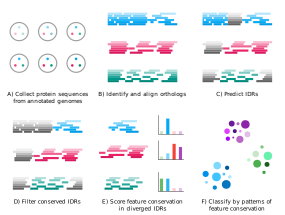
\includegraphics[width=\textwidth]{out/aims_overview.png}
\centering
\caption{\textbf{Graphical overview of aims.}
\textbf{(A)} The large open circles represent the genomes of different \textit{Drosophila} species, and the small, filled circles represent protein sequences in those genomes. Orthologs are colored with shades of the same hue. \textbf{(B-D)} Each horizontal line represents a sequence in panel A, and together each set of lines creates an ``alignment.'' The lines are broken where ``gaps'' are inserted to align equivalent segments. The grey segments denote regions of the alignment which are not part of subsequent analyses. \textbf{(E)} Each aligned IDR is scored on four features, where the ``strength'' of that feature is indicated by the height and color of its bar. \textbf{(F)} Scoring many IDRs on these features yields three distinct clusters.}
\label{fig:aims_overview}
\end{figure}

These comparisons, however, require the identification of IDRs with common ancestry that perform ``equivalent'' functions across many distinct organisms. Given the difficulties with identifying similar IDRs by their sequences, this may seem like a chicken and egg problem. Fortunately, IDRs are frequently associated with more conserved folded domains. Thus, identifying evolutionarily related proteins by their overall sequence signatures and ``aligning'' them will in turn identify the equivalent IDRs in those sequences. The first step of an evolutionary analysis of IDRs, then, is the identification of proteins with common ancestry, called orthologs. Since the first genomes were sequenced in the late 1990s, researchers have developed techniques for identifying and aligning orthologs~\cite{Fleischmann1995, Goffeau1996, CESC1998, Tatusov1997}. While these methods are generally effective, they are conducted by automated computational pipelines and prone to errors when processing the highly divergent sequences that characterize many IDRs. The evolutionary relationships between the genomes of closely related species generally make such mistakes easier to identify, and fortunately over the past five years advances in DNA sequencing technology have yielded dramatic increases in the number of sequenced genomes in the \textit{Drosophila} genus. However, because the existing methods for ortholog identification were designed for fewer or more distantly related genomes, they do not fully leveraged the available genomic redundancy to minimize errors. Thus, in the first chapter I develop a novel method for identifying orthologs which addresses this shortcoming and apply it to 33 \textit{Drosophila} genomes to generate a set of aligned orthologs (Fig.~\ref{fig:aims_overview}A-B). In the second chapter I then identify rapidly evolving IDRs in these ``alignments'' and analyse them with a variety of evolutionary models to detect patterns of conservation (Fig.~\ref{fig:aims_overview}C-F). Finally, in the third chapter I discuss several software tools and tutorials for fitting statistical models to data, which were created while pursuing the previous aims.
